\documentclass[a4paper,12pt]{article} 

%paquetes
\usepackage{graphicx}
\usepackage[spanish]{babel} 
\usepackage[utf8]{inputenc}
\usepackage{textcomp}
\usepackage{amssymb}
\usepackage{amsmath}
\usepackage{float}
\usepackage{subfig}
\usepackage{listings}

%caracteristicas de paginas
\pdfpagewidth 8.5in
\pdfpageheight 11in
\setlength\oddsidemargin{-0,21in}
\setlength\evensidemargin{-0,21in}
\setlength\topmargin{-2cm}
\setlength\textwidth{7in}
\setlength\textheight{9in}
\setlength\parskip{0.1in}

%%%%%%%%%%%%%%%%%%%%%%%%%%%%%%%%%%%%%%%%%%%%%%%%%%%%%%%%%%%%%

\begin{document} 

\title{Introducci\'on a la soluci\'on num\'erica de ODE's \\
\large Gu\'ia computacional 1 - Mec\'anica Cl\'asica 2016 - Clase G. Mindlin}
\author{Ignacio Poggi - L.U: 567/07 - ignaciop.3@gmail.com}
\maketitle

%\tableofcontents  %lo ponemos para trabajo largos que necesiten indice


\section{Enunciado}

En la secci\'on de materiales adicionales de la c\'atedra se encuentra un programa principal y un integrador Runge-Kutta de orden 4 (rk4) en lenguaje C. En el programa principal se encuentra escrita una ecuaci\'on diferencial a integrar, los par\'ametros y las condiciones iniciales. Sobre este c\'odigo van a trabajar en las siguientes actividades realizando las modificaciones pertinentes para su problema en particular.

En ubuntu es posible compilar y ejecutar el c\'odigo directamente desde una terminal abierta en una carpeta que contenga tanto el programa principal como el integrador rk4:\newline

\framebox[1.1\width]{gcc ODE\_ejX.c -o ode\_ejX -lm rk4.c}

\framebox[1.1\width]{./ode\_ejX}\newline

Se obtendr\'a como salida un archivo llamado $ejX.dat$ , donde $X$ es el n\'umero del ejercicio, que contiene el resultado de la integraci\'on. Los resultados pueden ser analizados gr\'aficamente mediante un graficador, en nuestro caso utilizaremos \textbf{gnuplot} que se controla mediante comandos en terminal.\newline


{\Large \textbf{Actividad 1}}

Editar el c\'odigo de ODE.c para analizar los siguientes puntos:

\begin{itemize}
\item C\'omo var\'ia el resultado seg\'un el paso de integraci\'on. Programe una integraci\'on con el m\'etodo de Euler y compare.
\item Analizar c\'omo evoluciona el sistema dadas distintas condiciones iniciales.
\end{itemize}
Qu\'e tipo de conclusiones puede obtener a partir de los an\'alisis anteriormente realizados.\newline


{\Large \textbf{Actividad 2 - Oscilador arm\'onico amortiguado}}

El oscilador arm\'onico amotiguado es un problema del cual se conoce la soluci\'on anal\'itica cuya ecuaci\'on diferencial que rige el movimiento es:

\begin{equation}
	\frac{d^2 x}{dt^2} + 2\gamma\frac{dx}{dt} + \omega_0^2x = 0
\end{equation}

Estudie num\'ericamente las soluciones del sistema seg\'un la relaci\'on de los par\'ametros, para ello: escriba la ecuaci\'on de segundo orden como dos ecuaciones de primer orden, var\'ie $\gamma$ y $\omega$ e integre. Tambi\'en analice distintas condiciones iniciales. Compare con lo conocido de la soluci\'on anal\'itica, para ello grafique como evoluciona la posici\'on en el tiempo, la velocidad y cu\'al es la trayectoria en el espacio de fases $x  \ddot{x}$.\newline


{\Large \textbf{Actividad 3 - Oscilador de Van der Pol}}

Es un tipo de oscilador con un amortiguamiento no lineal descripto a principio de siglo por Van der Pol quien estudi\'o circuitos el\'ectricos con componentes no lineales obteniendo la ecuaci\'on:

\begin{equation}
	\frac{d^2 x}{dt^2} + \mu(x^2-1)\frac{dx}{dt} + x = 0
\end{equation}

Este sistema presenta soluciones oscilatorias para ciertos valores del par\'ametro $\mu$ que son conocidas como oscilaciones de relajaci\'on. Esta ecuaci\'on tiene una importancia en la ciencia ya que fue usada en distintos campos para describir por ejemplo, el comportamiento de una falla tect\'onica o el potencial de acci\'on de una neurona. Esto se debe a que el sistema seg\'un los valores de $x$ presenta un amortiguamiento positivo (como el de la actividad 2 donde el sistema pierde energ\'ia), y para otros presenta un amortiguamiento "negativo" donde el sistema gana energ\'ia. Esto produce que eventualmente la energ\'ia perdida en un ciclo sea igual a la ganada generando oscilaciones autosostenidas. Este sistema se ver\'a con m\'as detalle avanzado el curso, en esta pr\'actica se propone realizar un acercamiento de forma num\'erica para tener cierta comprensi\'on de c\'omo se comporta el mismo.

\begin{itemize}
\item Escriba el sistema como dos ecuaciones de primer orden.
\item Inspeccione num\'ericamente las soluciones posibles del sistema, estudie como var\'ian seg\'un la variaci\'on del par\'ametro $\mu$. Para ello grafique la trayectoria $x$ en funci\'on del tiempo, la velocidad $\ddot{x}$ en funci\'on del tiempo y tambi\'en el espacio de fases $x  \ddot{x}$.
\item Modifique tambi\'en las condiciones iniciales y estudie num\'ericamente las respuestas del sistema. Para ello grafique la trayectoria $x$ en funci\'on del tiempo, la velocidad $\ddot{x}$ en funci\'on del tiempo y tambi\'en el espacio de fases $x  \ddot{x}$.
\end{itemize}


{\Large \textbf{A entregar}}

Se deber\'a entregar un trabajo de la actividad 2 y 3, con los c\'odigos, los gr\'aficos obtenidos para las integraciones num\'ericas propuestas y el correspondiente an\'alisis para cada caso.


\section{An\'alisis de datos y conclusiones}
\subsection{Oscilador arm\'onico amortiguado}

El oscilador arm\'onico amotiguado es el caso generalizado de los osciladores arm\'onicos libres ya que su comportamiento contempla la disipaci\'on de energ\'ia pero no la presencia de fuerzas externas. Su comportamiento est\'a dado por (1).
Para obtener las soluciones de dicha ecuaci\'on, se propone una con la forma $x(t) = e^{zt}$, con $z \in \mathbb{C}$ (luego $\dot{x}(t) = ze^{zt}$ y $\ddot{x}(t) = z^2e^{zt}$).

Reemplazando el $x(t)$ y sus derivadas en (1), se obtiene la siguiente ecuaci\'on cuadr\'atica para $z$:

$$
(z^2 + 2\gamma z + \omega_o^2)e^{zt}=0
$$

Esta ecuaci\'on es igual a 0 si y solo si $(z^2 + 2\gamma z + \omega_o^2) = 0$. Las ra\'ices de este polinomio son:

$$
z_{1,2} = \frac{-2\gamma \pm \sqrt{4\gamma^2 - 4\omega_0^2}}{2} = -\gamma \pm \sqrt{\gamma^2 - \omega_0^2}
$$

Podemos distinguir tres casos que, a continuaci\'on, analizamos por separado.

\begin{itemize}
\item Si $\omega_0^2 > \gamma^2$, tenemos dos raices complejas
$$z_{1} = -\gamma + i\sqrt{\omega_0^2 - \gamma^2}$$  $$z_{2} = -\gamma - i\sqrt{\omega_0^2 - \gamma^2}$$
Sea $\omega_{1} = \sqrt{\omega_0^2 - \gamma^2}$. Reemplazando esta nueva frecuencia en la soluci\'on propuesta y tomando su parte real, tenemos que:
\begin{equation}
x(t) = e^{-\gamma t}(acos(\omega_{1}t) + bsin(\omega_{1}t))
\end{equation}

$$\dot{x}(t) = e^{-\gamma t}((\omega_{1}b - \gamma a)acos(\omega_{1}t) + (\omega_{1}a - \gamma b)bsin(\omega_{1}t))$$

donde $a$ y $b$ se determinan con las condiciones iniciales
$$ x(0) = a, \dot{x}(0) = \omega_{1}b - \gamma a$$
Luego, la ecuaci\'on (3) nos queda:
\begin{equation}
x(t) = e^{-\gamma t}(x(0)cos(\omega_{1}t) + \frac{\dot{x}(0) + \gamma x(0)}{\omega_{1}}sin(\omega_{1}t))
\end{equation}

Este movimiento corresponde a una oscilaci\'on arm\'onica de frecuencia $\omega_{1}$, diferente de la frecuencia natural $\omega_{0}$; y se denomina \textit{movimiento oscilatorio subamortiguado}.

\begin{figure}[H]
\begin{center}
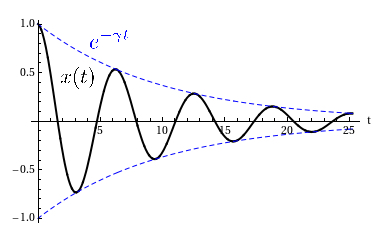
\includegraphics[height=8cm]{oscilacion_subamortiguada.jpg}
\caption[width=5cm]{Movimiento oscilatorio subamortiguado.\newline Se observa como la curva esta modulada por un termino exponencial relacionado con la constante de amortiguamiento $\gamma$.}
\end{center}
\end{figure}

\item Si $\omega_0^2 < \gamma^2$, tenemos dos raices reales
$$z_{1} = -\gamma + \sqrt{\gamma^2 - \omega_0^2}$$  $$z_{2} = -\gamma - \sqrt{\gamma^2 - \omega_0^2}$$


En este caso, la ecuaci\'on $x(t)$ nos quedar\'a expresada en t\'erminos de cosenos y senos hiperb\'olicos. Para las condiciones iniciales procedemos como en el caso del oscilador subamortiguado, por lo tanto la ecuaci\'on de movimiento nos queda:

\begin{equation}
x(t) = x(0)e^{-\gamma t}cosh(\sqrt{\gamma^2 - \omega_0^2}t) + \frac{\dot{x}(0) + \gamma x(0)}{\sqrt{\gamma^2 - \omega_0^2}}e^{-\gamma t}sinh(\sqrt{\gamma^2 - \omega_0^2}t)
\end{equation}

Este movimiento se denomina \textit{oscilatorio sobreamortiguado}.

\begin{figure}[H]
\begin{center}
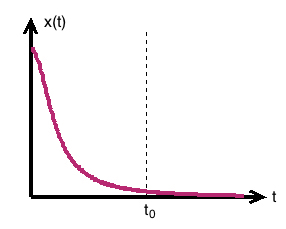
\includegraphics[height=8cm]{oscilacion_sobreamortiguada.jpg}
\caption[width=5cm]{Esquema del movimiento oscilatorio sobreamortiguado. En $t_{0}$ el sistema decae a 0 sin llegar a completar un periodo de oscilaci\'on.}
\end{center}
\end{figure}


\item Si $\omega_0^2 = \gamma^2$, tenemos una ra\'iz real doble

$$z_{1,2} = -\gamma$$

Al tener una \'unica ra\'iz doble, debemos considerar soluciones del siguiente tipo: 

$$ x(t) = (a+bt)e^{-\gamma t}$$

Al imponer las condiciones iniciales sobre $x(t)$, la soluci\'on nos queda:

\begin{equation}
x(t) = [x(0) + (\dot{x}(0) + \gamma x(0))t]e^{-\gamma t}
\end{equation}

Este movimiento se denomina \textit{oscilatorio con amortiguamiento cr\'itico}.

\begin{figure}[H]
\begin{center}
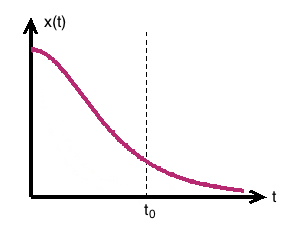
\includegraphics[height=8cm]{oscilacion_amortiguada_c.jpg}
\caption[width=5cm]{Esquema del movimiento oscilatorio con amortiguamiento cr\'itico.}
\end{center}
\end{figure}

\end{itemize}

Para el an\'alisis num\'erico, se reescribi\'o la ecuaci\'on de segundo orden (1) como dos ecuaciones de primer orden de la siguiente manera:

$$ \begin{cases} \dot{x} = y \\ \dot{y} = -2\gamma y - \omega_0^2 x \end{cases} $$

Este sistema se implemento en el c\'odigo fuente \textit{ODE\_ej2.c} (ver secci\'on Ap\'endice). Se utiliz\'o una variable \textit{j} dentro del bucle \textit{for} para ir iterando los distintos valores de $\gamma$ y $\omega_0$, as\'i como tambi\'en las condiciones iniciales $x(0)$ y $\dot{x}(0)$; desde $j$ = 1 hasta \textit{j} = 10. El tiempo m\'aximo de muestreo fue de 2 segundos.

Para destacar los casos sobre, sub y amortiguado cr\'itico, es necesario aclarar que se utilizaron incrementos de dicha variable con un valor igual a 4, por lo tanto \textit{j} solo toma 3 valores durante la ejecuci\'on del programa: \textit{j} = 1, \textit{j} = 5 y \textit{j} = 9; obteniendo una representaci\'on num\'erica y gr\'afica de los 3 casos mencionados anteriormente.

En el siguiente cuadro se pueden ver los valores num\'ericos para los par\'ametros y condiciones iniciales correspondientes a cada iteraci\'on:

\begin{table}
	\centering
    \begin{tabular}{ | l | l | l | l | l |p{5cm} |}
    \hline
    $j$ & $\gamma$ & $\omega_0$ & $x(0)$ &  $\dot{x}(0)$ \\ \hline
    1 & 9 & 1 & 0.5 & 4.5 \\ \hline
    5 & 5 & 5 & 2.5 & 2.5 \\ \hline
    9 & 1 & 9 & 4.5 & 0.5 \\
    \hline
    \end{tabular}
    \caption{Valores de los par\'ametros $\gamma$, $\omega_0$ y las condiciones iniciales en cada iteraci\'on. La primera fila corresponde al caso sobreamortiguado ($\gamma^2 > \omega_0^2$), la segunda al caso de amortiguamiento cr\'itico ($\gamma^2 = \omega_0^2$) y la tercera al caso subamortiguado ($\gamma^2 < \omega_0^2$).}
    \label{table:1}
\end{table}
\newpage


Los gr\'aficos correspondientes a estos resultados son los siguientes:

\begin{figure}[H]
\begin{center}
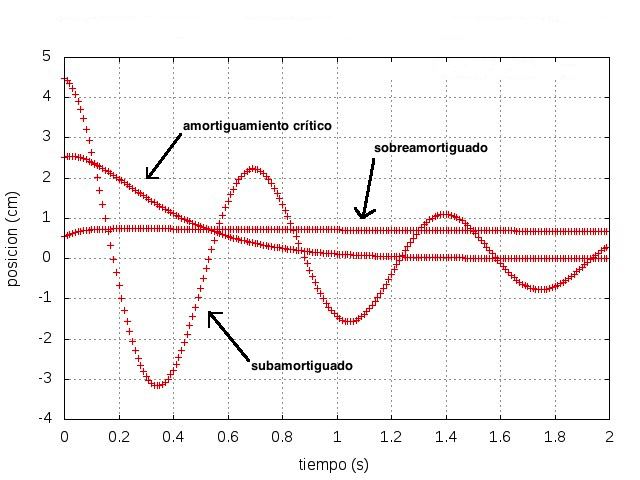
\includegraphics[height=8cm]{grafico_ej2_xVSt.jpg}
\caption[width=5cm]{Posici\'on en funci\'on del tiempo para los 3 casos estudiados del oscilador arm\'onico amortiguado.}
\end{center}
\end{figure}

\begin{figure}[H]
\begin{center}
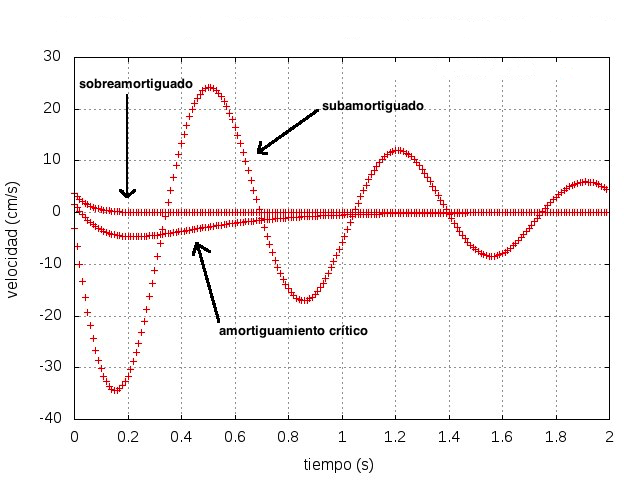
\includegraphics[height=8cm]{grafico_ej2_vVSt.jpg}
\caption[width=5cm]{Velocidad en funci\'on del tiempo para los 3 casos estudiados del oscilador arm\'onico amortiguado.}
\end{center}
\end{figure}

\begin{figure}[H]
\begin{center}
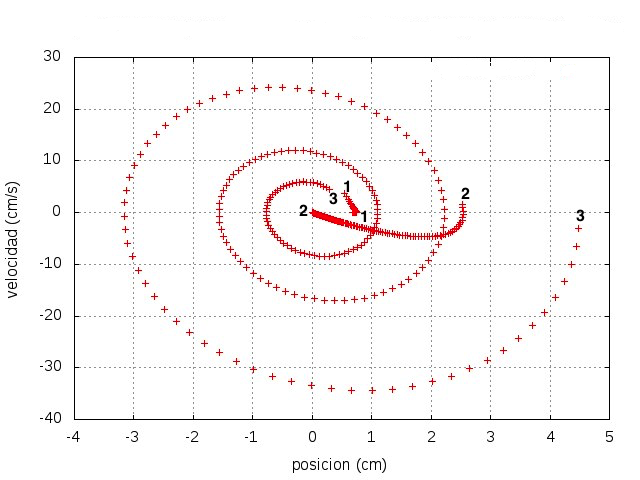
\includegraphics[height=8cm]{grafico_ej2_xVSv.jpg}
\caption[width=5cm]{Espacio de fases para los 3 casos estudiados del oscilador arm\'onico amortiguado.}
\end{center}
\end{figure}

Se observa en los gr\'aficos que el integrador de Runge-Kutta de orden 4 provisto por la c\'atedra, y los valores escogidos para destacar los 3 casos, aproximan satisfactoriamente a las soluciones anal\'iticas del oscilador arm\'onico amortiguado detalladas en la introducci\'on te\'orica del mismo.

Tambi\'en podemos ver que, en el caso sobreamortiguado, como $\gamma^2$ = 81 y $\omega_0^2$ = 1, el amortiguamiento es excesivo frente a la oscilaci\'on natural del sistema, por lo tanto la posici\'on y velocidad decaen muy rapidamente, sin llegar a 0. Esta situaci\'on en el espacio de fases esta representada por una linea muy corta, se\~nalada al principio y al final con el numero 2.

Para el caso de amortiguamiento cr\'itico, $\gamma^2$ = $\omega_0^2$ = 25, la funci\'on $x(t)$ presenta un decaimiento exponencial, similar al caso sobreamortiguado. En un oscilador de estas caracter\'isticas, el retorno a la posici\'on de equilibrio se da r\'apidamente. En el espacio de fases se puede ver como la linea gruesa marcada con el numero 1 al principio y al final de la misma.

En el caso subamortiguado, $\gamma^2$ = 1 y $\omega_0^2$ = 81. Esto se ve reflejado en una gr\'afica cosenoidal con una envolvente exponencial que decae mas lentamente que en los otros dos casos, y se hace 0 en un tiempo mas largo que el tiempo de muestreo de 2 segundos. \newline
Se observa adem\'as la gran amplitud y frecuencia inicial de esta funci\'on con respecto a los casos sobreamortiguado y amortiguado cr\'itico, debido a los valores de ${x}(0)$ y $\omega_0^2$ asignados a este caso. En el espacio de fases se puede ver como la curva marcada al principio y al final con el numero 3.


\subsection{Oscilador de Van der Pol}

Para realizar el an\'alisis num\'erico de este oscilador no-lineal, se reescribi\'o la ecuaci\'on de segundo orden (2) como dos ecuaciones de primer orden utilizando las ecuaciones de Li\'enard:

$$ \begin{cases} \dot{x} = \mu (y-(x^3-x)) \\ \dot{y} = -\frac{1}{\mu}x \end{cases} $$

Podemos destacar dos reg\'imenes interesantes para este oscilador, dependientes del par\'ametro $\mu$:

\begin{itemize}
\item Si $\mu$ = 0, no hay amortiguamiento y la ecuaci\'on (2) queda:
$$ \frac{d^2 x}{dt^2} + x = 0 $$
Es la f\'ormula del oscilador arm\'onico simple sin p\'erdida de energ\'ia.
\item Si $\mu$ $>$ 0, el sistema alcanzar\'a un ciclo l\'imite, en el que se conservar\'a la energ\'ia. Cerca del origen $x$ = $\frac{dx}{dt}$ = 0, el sistema es inestable; y lejos del origen hay amortiguamiento.
\end{itemize}

Este \'ultimo caso es el m\'as interesante y para el cual se analizaron num\'ericamente dos posibilidades: amortiguamiento muy peque\~no ($\mu$ $<<$ 1) y amortiguamiento muy grande ($\mu$ $>>$ 1)

Este sistema se implemento en el c\'odigo fuente \textit{ODE\_ej3.c} (ver secci\'on Ap\'endice). Se aumento el tiempo de muestreo a 20 segundos con respecto al ejercicio anterior, para poder ver detalladamente el espacio de fases de este oscilador.
Se decidi\'o graficar con l\'ineas continuas para facilitar la visualizaci\'on de la posici\'on, velocidad y espacio de fases de este oscilador.

\begin{itemize}
\item $\mu$ $<<$ 1:


En primera instancia, se dejaron las condiciones iniciales fijas ($x$(0) = -0.01 y $\dot{x}$(0) = 0.05). El par\'ametro $\mu$ toma los valores $\mu_1$ = 0.05 y $\mu_2$ = 0.005 en cada ejecuci\'on. 

\begin{figure}[H]
\begin{center}
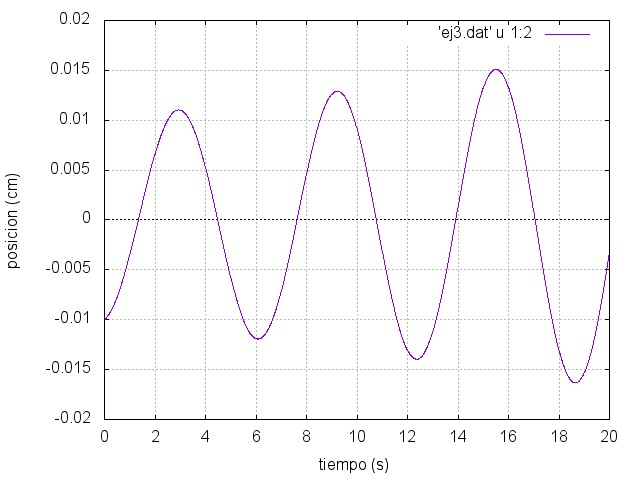
\includegraphics[height=8cm]{grafico_ej3_xVSt.jpg}
\caption[width=5cm]{Posici\'on en funci\'on del tiempo para $\mu_1$ = 0.05 y condiciones iniciales fijas.}
\end{center}
\end{figure}

\begin{figure}[H]
\begin{center}
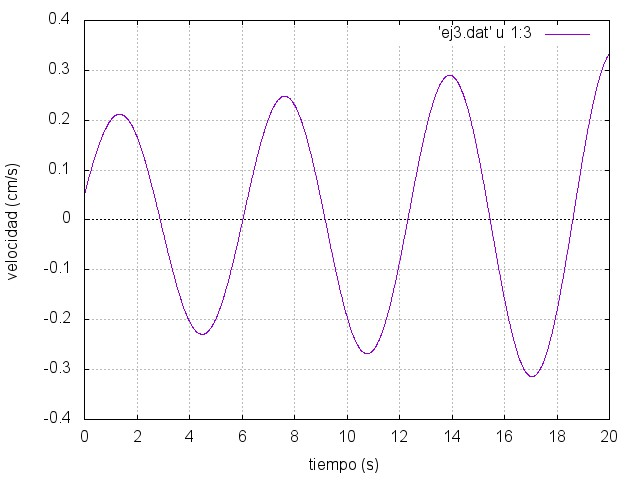
\includegraphics[height=8cm]{grafico_ej3_vVSt.jpg}
\caption[width=5cm]{Velocidad en funci\'on del tiempo para $\mu_1$ = 0.05 y condiciones iniciales fijas.}
\end{center}
\end{figure}

\begin{figure}[H]
\begin{center}
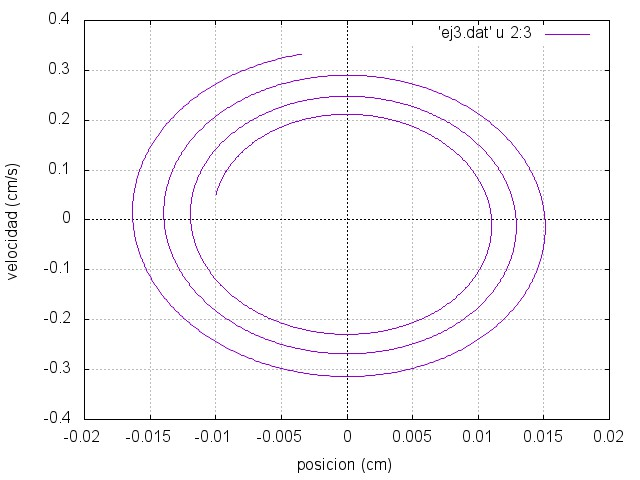
\includegraphics[height=8cm]{grafico_ej3_xVSv.jpg}
\caption[width=5cm]{Espacio de fases para $\mu_1$ = 0.05 y condiciones iniciales fijas.}
\end{center}
\end{figure}

\begin{figure}[H]
\begin{center}
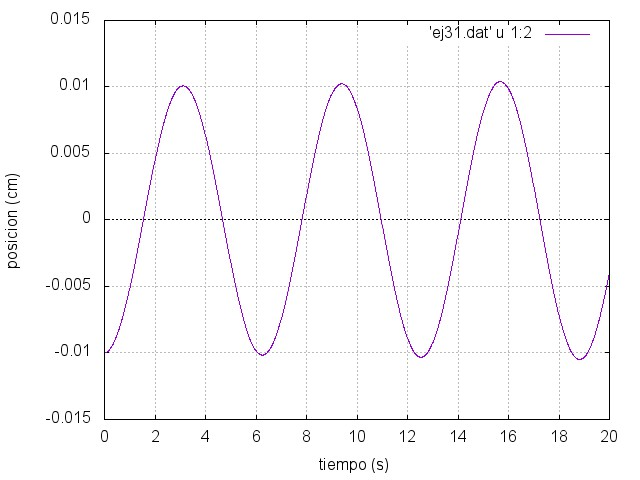
\includegraphics[height=8cm]{grafico_ej31_xVSt.jpg}
\caption[width=5cm]{Posici\'on en funci\'on del tiempo para $\mu_2$ = 0.005 y condiciones iniciales fijas.}
\end{center}
\end{figure}

\begin{figure}[H]
\begin{center}
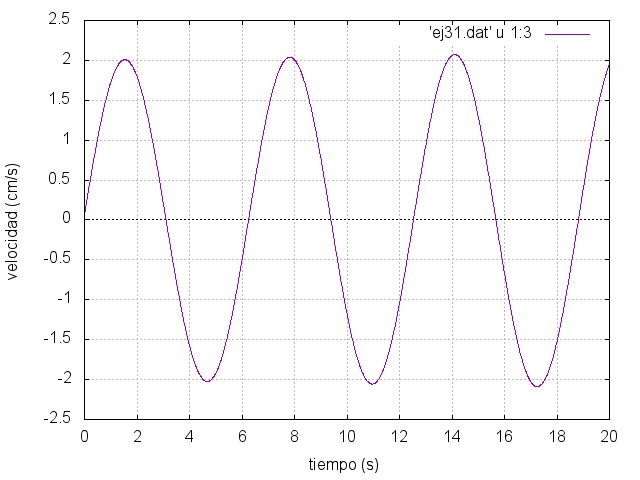
\includegraphics[height=8cm]{grafico_ej31_vVSt.jpg}
\caption[width=5cm]{Velocidad en funci\'on del tiempo para $\mu_2$ = 0.005 y condiciones iniciales fijas.}
\end{center}
\end{figure}

\begin{figure}[H]
\begin{center}
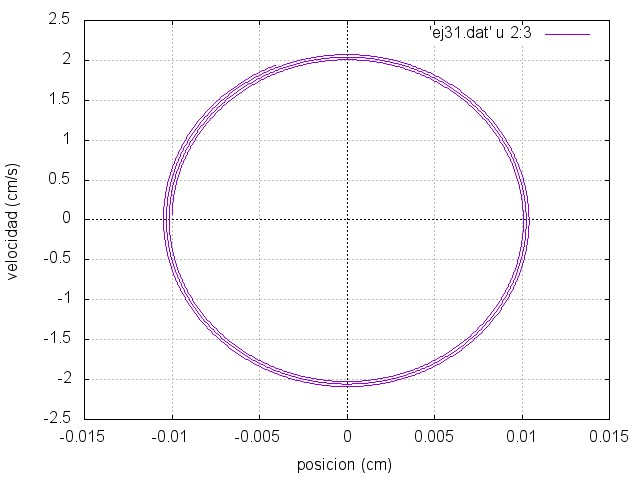
\includegraphics[height=8cm]{grafico_ej31_xVSv.jpg}
\caption[width=5cm]{Espacio de fases para $\mu_2$ = 0.005 y condiciones iniciales fijas.}
\end{center}
\end{figure}

Podemos observar que, con estos valores de $\mu$, el sistema se comporta como un oscilador armonico; sobre todo en el caso $\mu_2$ = 0.005.

MAS ANALISIS...


En una segunda instancia, las condiciones iniciales se variaron dentro de un bucle \textit{for}, esta vez con un iterador \textit{j} incrementado de a 1, con los mismos valores de $\mu_1$ y $\mu_2$. La siguiente tabla muestra los valores correspondientes a este caso:

\begin{table}
	\centering
    \begin{tabular}{| l | l | l | l | l | l | l | l | l | l |p{1cm}|}
    \hline
    \textit{j} & 1 & 2 & 3 & 4 & 5 & 6 & 7 & 8 & 9 & 10 \\ \hline
    $x(0)$ & 0.2 & 0.4 & 0.6 & 0.8 & 1 & 1.2 & 1.4 & 1.6 & 1.8 & 2 \\ \hline
    $\dot{x}(0)$ & -0.2 & -0.4 & -0.6 & -0.8 & -1 & -1.2 & -1.4 & -1.6 & -1.8 & -2 \\
    \hline
    \end{tabular}
    \caption{Condiciones iniciales en cada iteraci\'on para valores de $\mu_1$ = 0.05 y $\mu_2$ = 0.005.}
    \label{table:2}
\end{table}



\begin{figure}[H]
\begin{center}
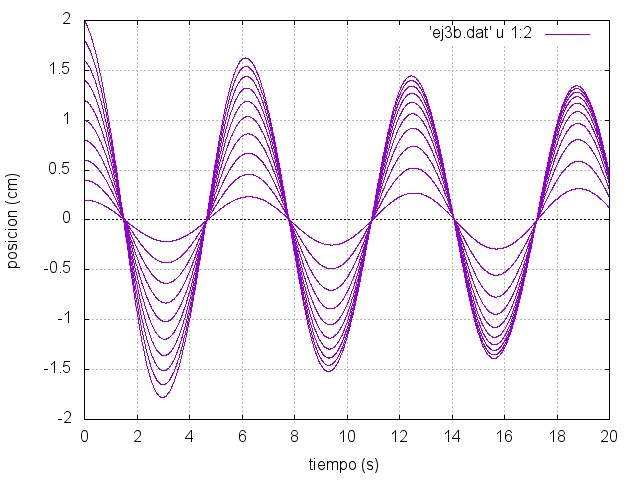
\includegraphics[height=8cm]{grafico_ej3b_xVSt.jpg}
\caption[width=5cm]{Posici\'on en funci\'on del tiempo para $\mu_1$ = 0.05 y condiciones iniciales variables.}
\end{center}
\end{figure}

\begin{figure}[H]
\begin{center}
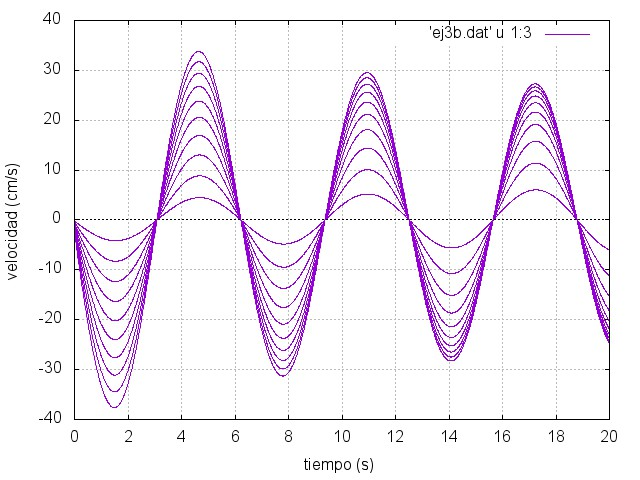
\includegraphics[height=8cm]{grafico_ej3b_vVSt.jpg}
\caption[width=5cm]{Velocidad en funci\'on del tiempo para $\mu_1$ = 0.05 y condiciones iniciales variables.}
\end{center}
\end{figure}

\begin{figure}[H]
\begin{center}
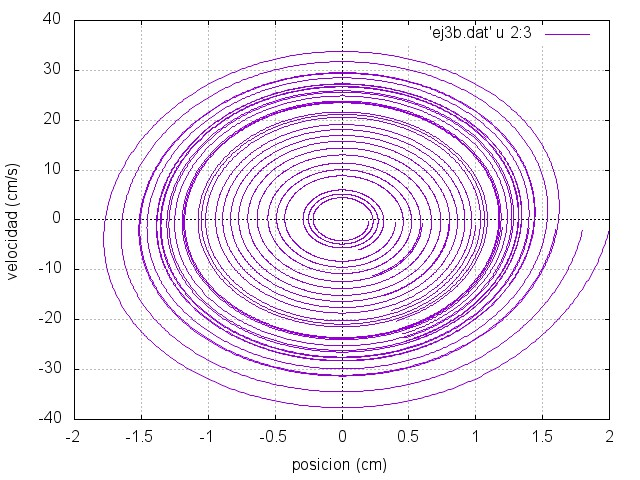
\includegraphics[height=8cm]{grafico_ej3b_xVSv.jpg}
\caption[width=5cm]{Espacio de fases para $\mu_1$ = 0.05 y condiciones iniciales variables.}
\end{center}
\end{figure}

\begin{figure}[H]
\begin{center}
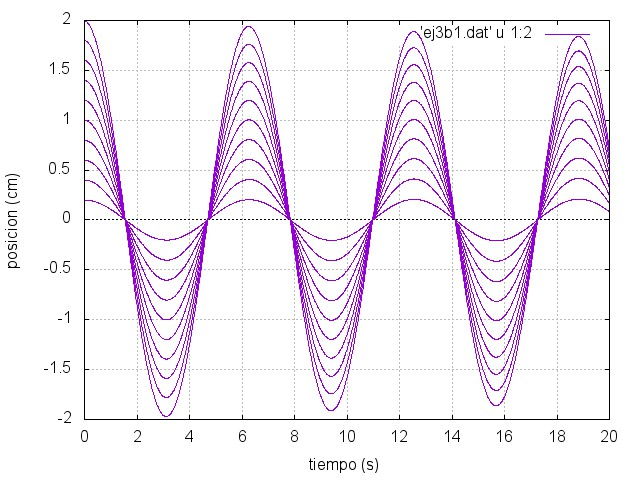
\includegraphics[height=8cm]{grafico_ej3b1_xVSt.jpg}
\caption[width=5cm]{Posici\'on en funci\'on del tiempo para $\mu_2$ = 0.005 y condiciones iniciales variables.}
\end{center}
\end{figure}

\begin{figure}[H]
\begin{center}
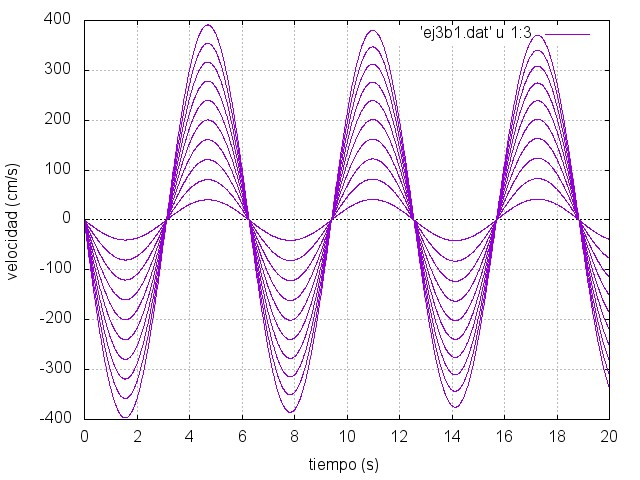
\includegraphics[height=8cm]{grafico_ej3b1_vVSt.jpg}
\caption[width=5cm]{Velocidad en funci\'on del tiempo para $\mu_2$ = 0.005 y condiciones iniciales variables.}
\end{center}
\end{figure}

\begin{figure}[H]
\begin{center}
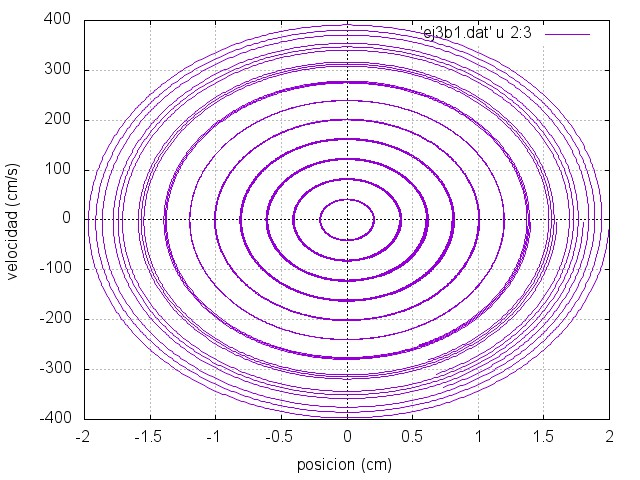
\includegraphics[height=8cm]{grafico_ej3b1_xVSv.jpg}
\caption[width=5cm]{Espacio de fases para $\mu_2$ = 0.005 y condiciones iniciales variables.}
\end{center}
\end{figure}

MAS ANALISIS....
------------------------------------


\item $\mu$ $>>$ 1:


Como en el caso anterior, primero se dejaron las condiciones iniciales fijas ($x$(0) = -0.01 y $\dot{x}$(0) = 0.05), variando el par\'ametro $\mu$ en cada ejecuci\'on por separado. ($\mu_1$ = 5 y $\mu_2$ = 10). Los graficos de posicion, velocidad y espacio de fases para dichos $\mu$ son los siguientes:

\begin{figure}[H]
\begin{center}
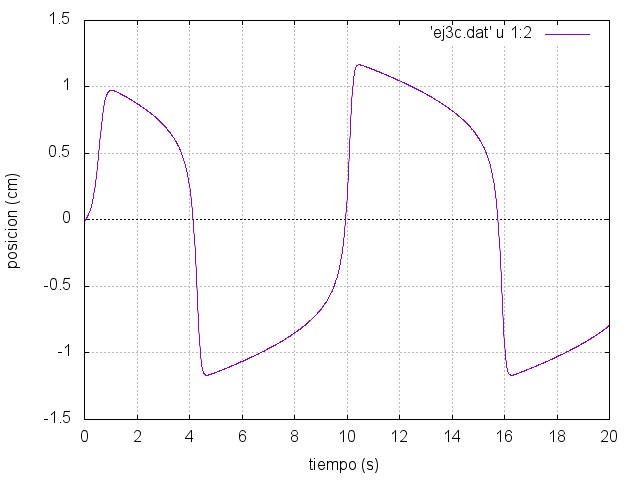
\includegraphics[height=8cm]{grafico_ej3c_xVSt.jpg}
\caption[width=5cm]{Posici\'on en funci\'on del tiempo para $\mu_1$ = 5 y condiciones iniciales fijas.}
\end{center}
\end{figure}

\begin{figure}[H]
\begin{center}
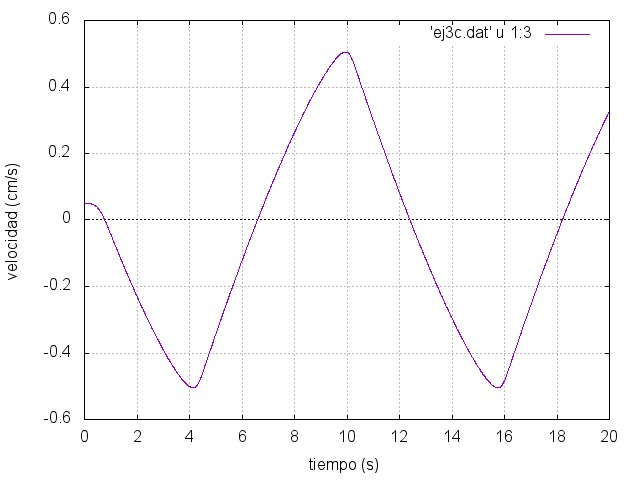
\includegraphics[height=8cm]{grafico_ej3c_vVSt.jpg}
\caption[width=5cm]{Velocidad en funci\'on del tiempo para $\mu_1$ = 5 y condiciones iniciales fijas.}
\end{center}
\end{figure}

\begin{figure}[H]
\begin{center}
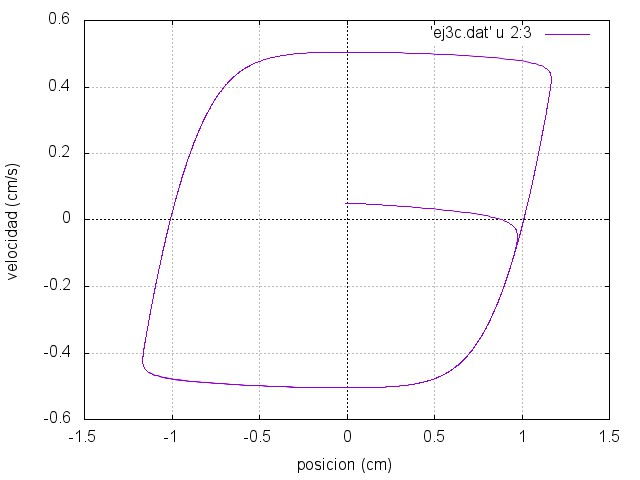
\includegraphics[height=8cm]{grafico_ej3c_xVSv.jpg}
\caption[width=5cm]{Espacio de fases para $\mu_1$ = 5 y condiciones iniciales fijas.}
\end{center}
\end{figure}

\begin{figure}[H]
\begin{center}
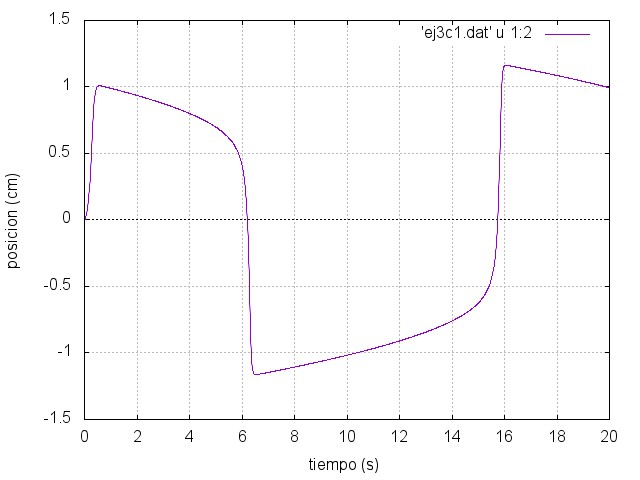
\includegraphics[height=8cm]{grafico_ej3c1_xVSt.jpg}
\caption[width=5cm]{Posici\'on en funci\'on del tiempo para $\mu_2$ = 10 y condiciones iniciales fijas.}
\end{center}
\end{figure}

\begin{figure}[H]
\begin{center}
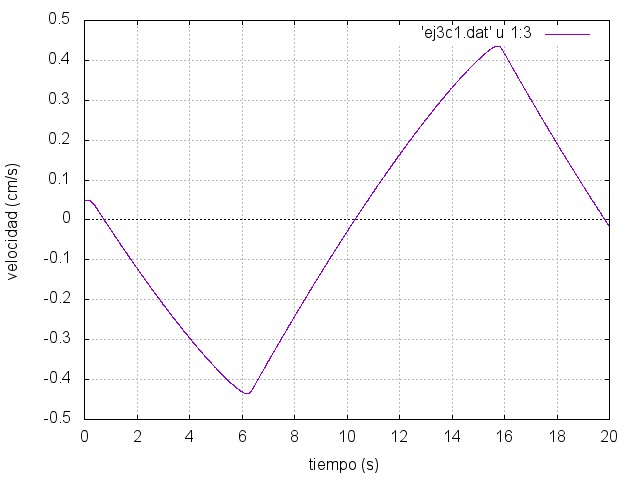
\includegraphics[height=8cm]{grafico_ej3c1_vVSt.jpg}
\caption[width=5cm]{Velocidad en funci\'on del tiempo para $\mu_2$ = 10 y condiciones iniciales fijas.}
\end{center}
\end{figure}

\begin{figure}[H]
\begin{center}
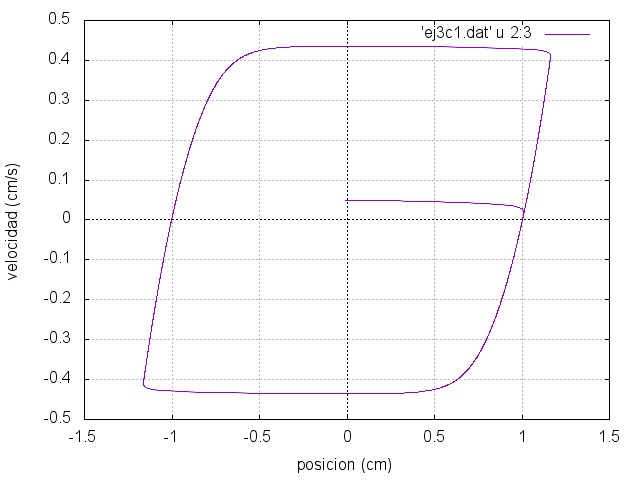
\includegraphics[height=8cm]{grafico_ej3c1_xVSv.jpg}
\caption[width=5cm]{Espacio de fases para $\mu_2$ = 10 y condiciones iniciales fijas.}
\end{center}
\end{figure}




Finalmente, las condiciones iniciales tambi\'en se variaron dentro bucle for, con los mismos valores que muestra el cuadro (2). Los gr\'aficos para este caso son los siguientes:

\begin{figure}[H]
\begin{center}
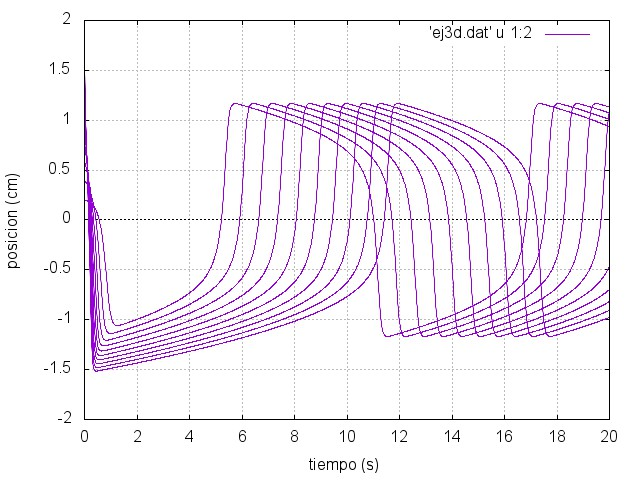
\includegraphics[height=8cm]{grafico_ej3d_xVSt.jpg}
\caption[width=5cm]{Posici\'on en funci\'on del tiempo para $\mu_1$ = 5 y condiciones iniciales variables.}
\end{center}
\end{figure}

\begin{figure}[H]
\begin{center}
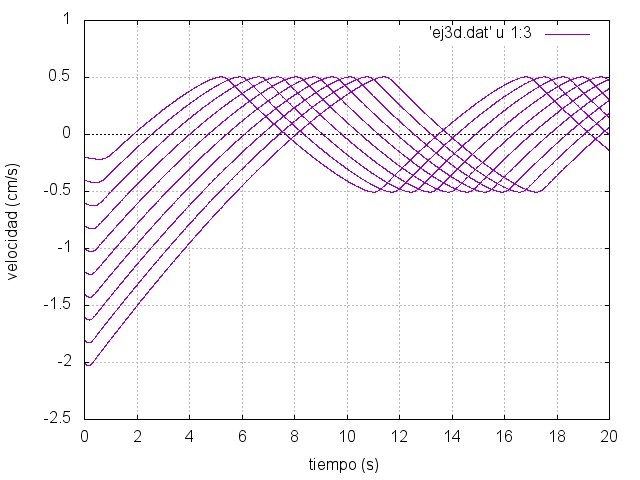
\includegraphics[height=8cm]{grafico_ej3d_vVSt.jpg}
\caption[width=5cm]{Velocidad en funci\'on del tiempo para $\mu_1$ = 5 y condiciones iniciales variables.}
\end{center}
\end{figure}

\begin{figure}[H]
\begin{center}
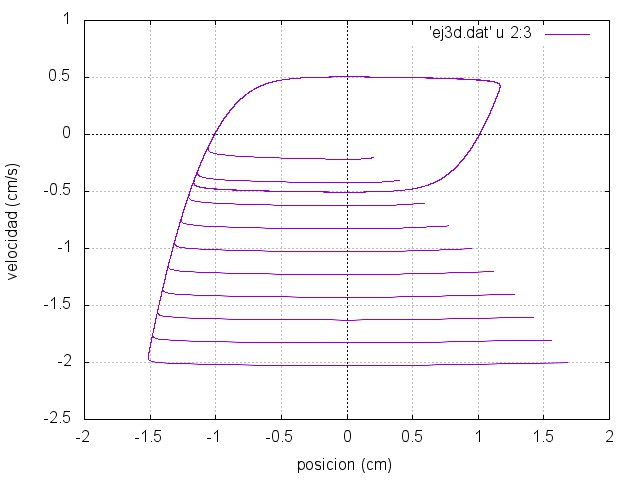
\includegraphics[height=8cm]{grafico_ej3d_xVSv.jpg}
\caption[width=5cm]{Espacio de fases para $\mu_1$ = 5 y condiciones iniciales variables.}
\end{center}
\end{figure}

\begin{figure}[H]
\begin{center}
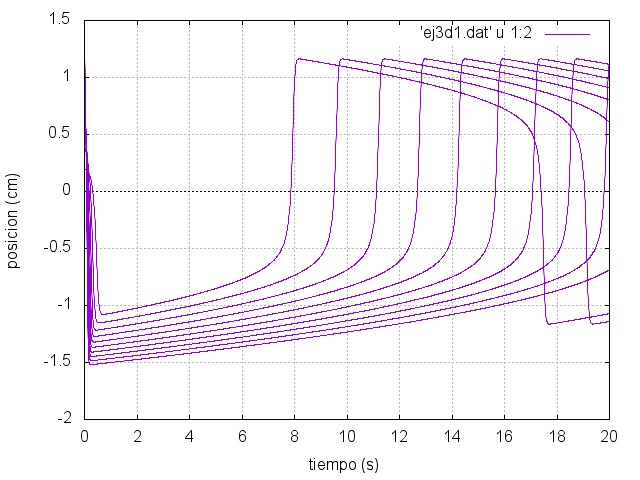
\includegraphics[height=8cm]{grafico_ej3d1_xVSt.jpg}
\caption[width=5cm]{Posici\'on en funci\'on del tiempo para $\mu_2$ = 10 y condiciones iniciales variables.}
\end{center}
\end{figure}

\begin{figure}[H]
\begin{center}
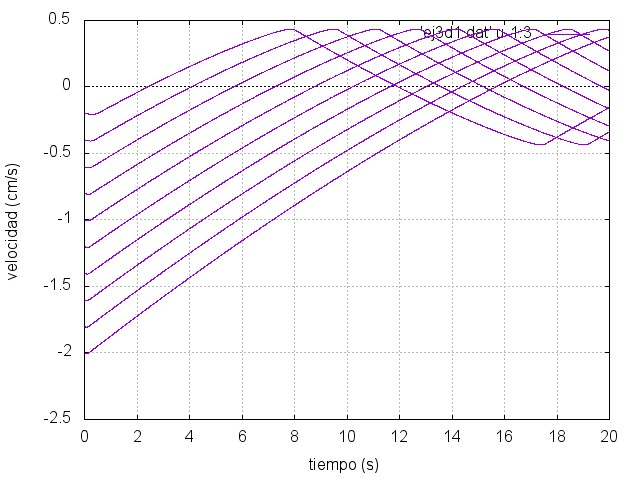
\includegraphics[height=8cm]{grafico_ej3d1_vVSt.jpg}
\caption[width=5cm]{Velocidad en funci\'on del tiempo para $\mu_2$ = 10 y condiciones iniciales variables.}
\end{center}
\end{figure}

\begin{figure}[H]
\begin{center}
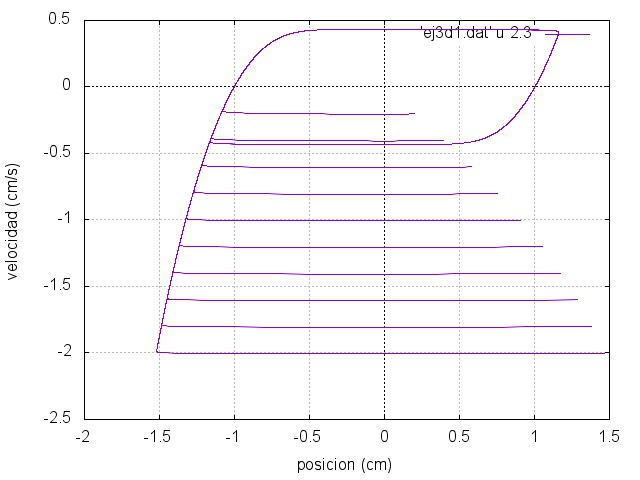
\includegraphics[height=8cm]{grafico_ej3d1_xVSv.jpg}
\caption[width=5cm]{Espacio de fases para $\mu_2$ = 10 y condiciones iniciales variables.}
\end{center}
\end{figure}

MAS ANALISIS.-------


\end{itemize}

\section{Ap\'endice}

Descargar el archivo $guia1\_poggi.zip$ y descomprimirlo en una carpeta a elecci\'on del usuario, abrir una terminal dentro de la carpeta $\sim \backslash mecanica-clasica\backslash practica1$; y seguir las instrucciones provistas en la secci\'on Enunciado.

Los archivos que contienen los datos num\'ericos $(ej2.dat$ y $ej3.dat)$ no fueron transcriptos en este informe dada la extensi\'on de los mismos.


\subsection{C\'odigo fuente en C del oscilador arm\'onico amortiguado (ODE\_ej2.c)}

\lstinputlisting[language=C,breaklines]{../ODE_ej2.c}

\subsection{C\'odigo fuente en C del oscilador de Van der Pol (ODE\_ej3.c)}
Se transcribi\'o un solo caso de este c\'odigo, las peque\~nas modificaciones para los casos restantes est\'an se\~nalados en el an\'alisis del oscilador.

\lstinputlisting[language=C,breaklines]{../ODE_ej3.c}

\subsection{C\'odigo fuente en C del m\'etodo de Runge-Kutta de orden 4 provisto por la c\'atedra (rk4.c)}
\lstinputlisting[language=C,breaklines]{../rk4.c}

\section{Bibliograf\'ia}




\end{document}
